\section{Overview}

In the last few decades we have learned that the brain does not process all incoming sensory information equally. According to our goals and context we filter out irrelevant information and select for sensory inputs that are important. At first, the idea that this filtering occurred in sensory cortex was a surprise-- but it is now generally accepted that changes in sensory representation drive selection.

In this thesis, I investigated the processes underlying selective visual attention in human cortex. The overarching goal was to establish how information is selected from visual representations for use during adaptable behavior. To do this, I started by extending an existing linking model of contrast, which controls the visibility of images, to a second feature: coherence. These two ways of manipulating the visibility of motion required a new framework to be built, demonstrating how visual cortex is sensitive to each of these features and whether they interact. I then connected this framework to perception. This connection, a computational linking model, allowed me to test different hypotheses about how perception depends on sensory representations. These models revealed that the scale of sensory changes due to attention were insufficient to capture perception, implicating a downstream readout process as a key component of selective visual attention. We expect these results to hold true for other forms of selection, e.g. by spatial location, color, or motion direction, and sought to demonstrate this in the final section of the thesis.

\subsection{Aim 1: Using linking models to compare implementations of selective visual attention}

The prevailing view is that attention is implemented by modifications of sensory responses. But without a computational linking model it is impossible to know whether these sensory changes are the only changes occurring during selective visual attention. 

\textbf{In Chapter 2, I build a quantitative framework for two features of motion visibility.} Contrast and motion coherence both control the visibility of motion and their representations in human visual cortex are similar. This makes them excellent tools to study whether sensory change alone can account for the behavioral effects of attention. In this chapter, I measure and quantify how these features are represented in human cortex to lay the ground work for a linking model.

\textbf{In Chapter 3, I use a linking model to show that sensory change is insufficient to account for all the behavioral effects of attention.} I first validate that a linking of motion visibility can be constructed, based on the quantitative framework developed in Chapter 2. Then, using the validated linking model I show that the sensory change occurring during selective visual attention is insufficient to account for behavioral changes -- a flexible readout must be a necessary component.

\subsection{Aim 2: Comparing different forms of sensory selection on a shared perceptual metric}

One question we asked ourselves after completing Aim 1, was whether our results would be consistent in other features. Is selection by motion visibility similar to selection by spatial location, by color, or by motion direction? Although we know that different visual features are processed in different ways, this does not necessarily mean that selection by these features requires different computational resources and implementations.

\textbf{In Chapter 4, I address this aim by building a psychophysics experiment with which I compare the strength of spatial and feature-based attention on a common metric.} I demonstrate in these experiments that the sensitivity (i.e. the variability in response error) is constant across different forms of selection. Given this similarity, this suggests that selection by color, motion direction, and location may all be implemented by similar mechanisms. I also present in this chapter preliminary results looking at how a computational linking model of color and motion direction estimation during selection might be constructed to connect these perceptual findings to measurements of human cortical activity. 

\break

Before going into detail about my experiments and computational models, I will review what is known about selective visual attention. In particular, I will focus on the history of how selection might be implemented as a computation in the human brain. Examples will be drawn from the existing literature on selection by spatial location, color, motion direction, and higher order features (such as faces or objects). I will also discuss the origin and existing uses of computational linking models, which are a key component of my research.

\section{Selective attention}

We all know, more or less intuitively, what it is like to attend to something that we see. When stopped at an intersection, a driver might be motivated by their context to focus on the direction of nearby cars, the movement of pedestrians, and the stop signs or traffic lights in their vicinity (Fig. \ref{fig:c0f1}a). The ease with which we can deploy attention hides a complex set of changes which occur inside the brain and which change our sensory perceptions. By moving such experiences into the laboratory we can operationalize them (Fig. \ref{fig:c0f1}b). That is to say, we can break down a complex process such as attention into the discrete changes which result from it. For example, attention might improve reaction times, detection, or the ability to discriminate between stimuli, but not necessarily all of these and not necessarily all to an equal extent. Once operationalized, we can begin to track the result of attending back to its roots inside of the brain.

\begin{figure}[ht]
\centering
\includegraphics[keepaspectratio,width=0.75\textwidth]{figs_c0/task_example.pdf}
\caption[Selective visual attention tasks]{Natural and operationalized tasks which engage selective visual attention. (a) A driver, stopped at an intersection, puts more contextual weight on information such as the direction of nearby cars, the movement of pedestrians, and stop signs or traffic lights in their vicinity. While those features of the visual environment might be enhanced, irrelevant information, like the colors of the sky or houses, might be filtered out of their perceptual experience. (b) To operationalize selective visual attention we simplify complex tasks like that presented in (a), to forms where the stimulus can be precisely manipulated. In this operationalized task, attention is used to select out two of the four dot patches and report their direction of motion. This allows us to compare different forms of attention: e.g. selection by color or by side.}
\label{fig:c0f1}
\end{figure}

\subsection{A brief history of selective attention research}

Attention research began from introspective observations of the experimenter's conscious experience. One of these early observations was that percepts become more "intense" or "clear" when focused upon \citep{Helmholtz1924-rl,James1981-cj,Kuelpe1902-qz,Titchener1908-bx}. Although intuiting changes in perceptions comes with many problems \citep{Helmholtz1924-rl}, these observations were not without merit. Spatial attention to some stimuli does appear to lead to a change in the appearance of a stimulus \citep{Carrasco2018-sb}. In fact, when carefully measured, it can be shown that these enhancements in perception trade off with a loss of information about ignored stimuli. Perhaps the earliest example of this is a set of experiments in which observers were asked to echo speech from one ear at a time \citep{Cherry1953-as}. Observers can do this, but they often recall little to no information about the ear they are asked to ignore, although some low-level details leak through such as the pitch of the speakers voice \citep{Cherry1953-as}. Together what these early findings revealed was that there is a common notion of \textit{attention} and it leads to a profound change in our conscious experiences. A vast literature has since been devoted to understanding how these changes occur as a function of neural activity in the brain. 

One of the changes necessary to go from intuition to an implementation-level understanding was to shift from intuition to objective measurement. The transition from introspection to ‘objective’ measurement can be highlighted in the way that the experiment mentioned above was introduced, quoting from \citet{Cherry1953-as}: ``the `subject' under test (the listener) is regarded as a transducer whose responses are observed when various stimuli are applied, whereas his subjective impressions are taken to be of minor importance''. This approach of seeing an observer as a kind of computational processor was effective. The field made an abrupt move toward understanding sensory systems as processing units and differentiating between the computations a system might employ versus the implementation of those computations \citep{Marr1982-fg}. The rough framework for how sensory processing occurs and how attention might interface with this is as follows: any given stimulus might be processed in a serial or parallel manner and processing might go to `completion' or be halted at a certain point, based on an observer's focus of attention. Measuring the knowledge of an observer about an attended or ignored stimulus therefore assesses the extent of processing which has occurred. For example, for the echoing task described earlier, an observer might be asked whether they had retained knowledge about an un-echoed (and therefore, unattended) voice. If they could recall simple low-level features, e.g. that the speaker had a higher-pitched voice, then a researcher could conclude that parallel processing of both streams had occurred up to pitch processing \citep{Cherry1953-as}. They could then also conclude that processing of the ignored stimulus had then been halted, before the point of complete semantic understanding. These kinds of results coincided with early findings about the human visual cortex \citep{Kuffler1953-qw,Hubel1962-pn,Hubel1968-na} which led researchers to begin to distinguish between stages of processing: an early parallel stage in which incoming sensory information is processed without immediate limits in capacity, and a second limited capacity serial stage from which complex decisions could be made. I'll discuss the physiology in more detail below, but first it is worth focusing on how attention might interface with these hypothetical processing stages. 

Several early theories of attention focused on when attentional selection might occur relative to the parallel and serial stages of processing. These theories fell out of the observations made above: some features of auditory stimuli (and other senses) are available for decision making regardless of the observers focus, while other features must be attended to be available. To reconcile these observations, researchers suggested a bottleneck and proposed that this was the mechanistic implementation of selective attention. The first such modern theory was Broadbent’s Filter theory \citep{Broadbent1958-ny}, which included an early bottleneck. In Filter theory, visual information is processed in parallel until low-level features (location, intensity, frequency) are resolved. At this point, parallel processing gives way to a serial ‘complete’ processing of object identity, form, etc. The alternative theory, late selection, suggests that processing occurs up to semantics in an unconscious parallel manner \citep{Deutsch1963-ac}. An example best illustrates the distinctions in these theories. Again, if an observer is echoing one speaker while ignoring a second, a late selection account predicts that a substantial amount of information is nevertheless available about the ignored voice. This is because late selection predicts that semantic-level processing of speech will occur regardless of sensory selection, leaving high-level information available to an observer. Evidence for this comes from experiments in which observers orient to highly salient but also very high-level features such as their own name, even when focused on other tasks \citep{Moray1959-fn}. These two theories have since been reconciled by suggesting two things: first, that not all features are processed in identical ways, and second that selection is either graded \citep{Treisman1960-qs} or has variable capacity limits at different stages \citep{Kahneman1973-af}.

This thesis is primarily focused on selective visual attention, but the results are likely to be broadly applicable to different forms of attention. Selective attention has been most heavily studied in the visual domain, in part because of the close relationship between selecting information in the world and orienting of the eyes. There are two ways to orient visual attention. An observer can make an overt movement of the eyes or they can covertly attend, without moving the eyes. Like all forms of selective attention, covert attention can accelerate responses \citep{Eriksen1972-qj,Posner1980-cr}, improve detection performance, and increase discrimination sensitivity \citep{Carrasco2011-xp}. Cues about important locations can both be imposed externally on an observer \citep{Posner1980-wb} or the result of internal guiding of attention toward a cued location. For the remainder of this introduction I will focus on covert visual attention and how researchers have suggested it might be implemented in human visual cortex.

\section{Organization of the human (and primate) visual cortex}

Before going into detail about how selective visual attention might operate over sensory representations I will introduce some background about how the human (and primate) visual cortex is organized. 

The selection of visual information is primarily thought to occur in cortex and not in the retina or in thalamic relay areas as visual signals project to cortex. Briefly, visual perception begins when light reaches the cones and rods in the retina. These photoreceptors transduce photons into electrical signals while maintaining spatial precision and implicitly coding information about wavelength. Substantial processing occurs in parallel within the retina by the many different retinal ganglion cells and related interneurons [cite: field/chichilnisky]. These cells then project their outputs to the lateral geniculate nucleus (LGN), a relay area within the thalamus. Again, considerable processing is known to occur within the LGN, and already in this second visual processing area modulation by attention is known to occur \citep{OConnor2002-mx}. It is in the LGN that visual information becomes contra-lateralized, i.e. the inputs from the two visual fields in each retina are separated and sent to the opposite hemispheres. The LGN sends its outputs into striate cortex area V1. Area V1 contains a full retinotopic map of the contralateral visual field and neurons in this area are sensitive to low-level features: contrast, spatial orientation and frequency, and color, among other simple visual features [todo: cite].

Area V1 sends its projections on to a multitude of retinotopic areas (V2, V3, etc) which together are referred to as ``early visual cortex''. These areas have progressively larger receptive fields \citep{Dumoulin2008-uc} and are sensitive to more complex features [todo: cite recent cnn work, e.g. seibert/yamins/gardner?]. Eventually, visual processing differentiates into at least two streams \citep{Mishkin1983-ys} which encode primarily for object identity or temporal information like motion. The ventral stream (hV4 and regions in ventral temporal cortex) is thought to encode information about the shape, color, and texture of objects. The dorsal stream (MT and posterior parietal cortex) are thought to encode information about spatial processing and depth. These broad definitions were based on lesion studies which showed a double dissociation where ventral temporal cortex lesions lead to deficits in pattern and object recognition but not grasping behaviors, and vice versa. All modern models of these processing streams acknowledge that they are far from distinct and are deeply interconnected.

In this thesis, I focus in particular on areas that are important for the processing of low-level visual features, such as contrast (area V1, orange shading Fig. \ref{fig:c0f2}) and motion coherence (area hMT+, purple shading Fig. \ref{fig:c0f2}). I demonstrate in this thesis that these areas are parametrically related to each of these properties, respectively, and importantly their responses are scaled in a manner which reflects human perception to each feature. Other areas that are likely involved in representing these features include V2, V3, V3A and V3B, hV4, and V7 -- all retinotopic areas in early visual cortex. In Aim 2, I focus on features such as color and motion, which also implicate similar parts of human visual cortex.

\begin{figure}[ht]
\centering
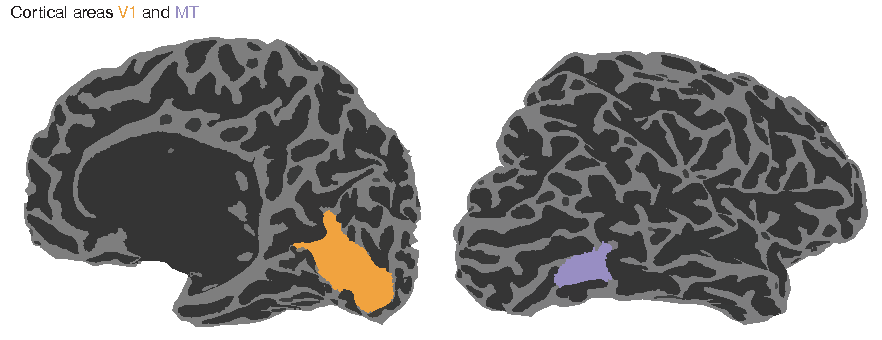
\includegraphics[keepaspectratio,width=0.75\textwidth]{figs_c0/brains.pdf}
\caption[Brain regions implicated in motion visibility perception]{Human cortical areas implicated in the representation and perception of motion visibility. Two brain areas in the human visual cortex: V1 and MT, are shown highlighted on a reconstructed cortical surface. These two regions are critical areas in the processing of motion visibility, the main stimulus feature studied in this thesis.}
\label{fig:c0f2}
\end{figure}

\section{Implementations of selective visual attention}

Selective attention is a balancing act for the brain, which must weigh the possibility of needing unattended information against the strength of sensory selection. In an early selection theory, information is being thrown out before complete processing -- which could be potentially disadvantageous if that stimulus later becomes important for behavior \citep{Mack1998-nq}. In fact, any modification of sensory representations to enhance one visual feature will have a cost for others. Attention research has always been aware of this and in a few particularly dramatic demonstrations \citep{Haines1991-si,Mack1998-nq,Neisser1979-mm,Simons1999-ng} observers can be shown to entirely lose access to otherwise highly salient information. These selection effects require observers to be performing a task with significant cognitive load \citep{Lavie2005-aw,Lavie2004-ub,Rees1997-hd}. Because much of the information that is selected out can still be found in early visual cortex [todo: cite] it seems clear that the implementation of selective visual attention involves the gating of information transfer between cortical areas. Finding where and when this gating computation occurs is a primary goal for the study of selective visual attention. 

Modern neuroscience now deploys a multitude of neural recording techniques to understand how sensory selection might be implemented by the brain. Both at a coarse scale in humans and at the level of individual neurons in primates and, very recently, rodents. In humans and non-human primates attention has been shown to alter the response gain of neurons in the visual system, including in the LGN \citep{OConnor2002-mx}, in V1 \citep{Motter1993-av}, V2 \citep{Buffalo2010-lr,Luck1997-sq,Motter1993-av}, V3 \citep{Liu2007-jx,Pestilli2011-gi,Saenz2002-fs,Silver2007-vd}, V4 \citep{Buffalo2010-lr,Connor1996-nm,Luck1997-sq,McAdams1999-jy,Moran1985-cv,Motter1993-av,Reynolds2000-mg,Spitzer1988-ib}, V3A \citep{Serences2007-le},  MT \citep{Beauchamp1997-rh,OCraven1997-ej,Saenz2002-fs,Seidemann1999-oz,Serences2007-le,Treue1999-mp,Treue1996-ez} and MST \citep{OCraven1997-ej,Treue1996-ez}, and in IT cortex \citep{Chelazzi1998-gx,Moran1985-cv}. Using BOLD imaging these changes can be observed simultaneously throughout almost all of early visual cortex \citep{Liu2007-jx,Pestilli2011-gi,Saenz2002-fs,Silver2007-vd} and ventral temporal cortex \citep{Baldauf2014-uj}. Changes to sensory representations occur for spatial attention tasks \citep{Klein2014-oe,McAdams1999-jy,Mitchell2009-do,Pestilli2011-gi,Womelsdorf2006-np} and are thought to be linked to the preparation of saccades, perhaps originating from the frontal eye fields \citep{Moore2003-fs}. Sensory representations can also be modified in  feature-based attention tasks \citep{Baldauf2014-uj,Harel2014-wd,Huk2000-uj,Jehee2011-mb,Saenz2002-fs,Saenz2003-qz,Serences2007-le,Treue1999-mp}.

\begin{figure}[ht]
\centering
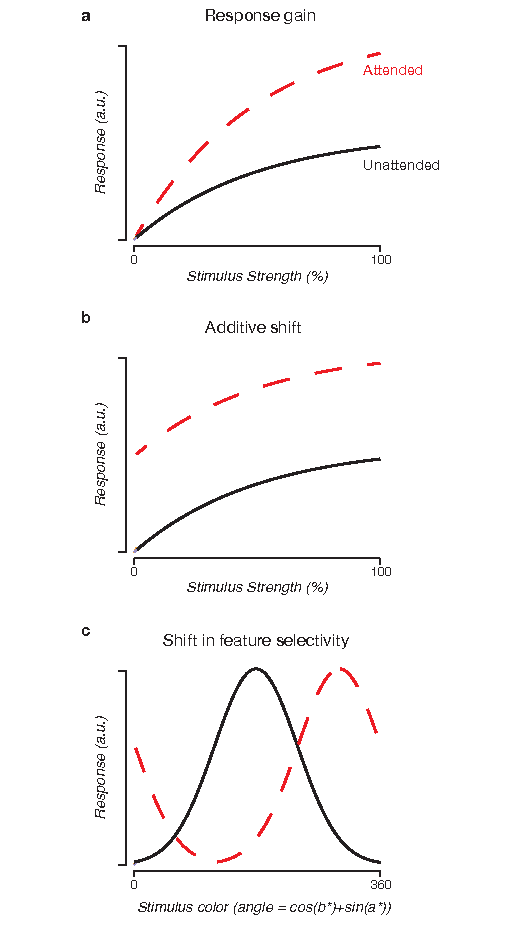
\includegraphics[keepaspectratio,width=0.5\textwidth]{figs_c0/attention_models.pdf}
\caption[Sensory implementations of attention]{Implementations of attention in sensory representations. (a) Multiplicative gain of the sensitivity of neurons during attention to a preferred feature. (b) An additive shift in the neural response, which could be used by a downstream mechanism to differentiate attended and unattended features. (c) A shift in the preferred feature of a neuron to a different feature.}
\label{fig:c0f3}
\end{figure}

From the observations made in these studies researchers have generated a few general hypotheses for how sensory representations might be modified during selective visual attention (Fig. \ref{fig:c0f3}). On early hypothesis was that neurons sensitive to an attended feature might become more sensitive during a selection behavior \citep{Reynolds2000-mg,Serences2007-le,Snyder2018-yr,Treue1999-mp} (Fig. \ref{fig:c0f3}a). Another possibility is that neurons increase their baseline response \citep{Buracas2007-pe,Chen2012-fu,Fang2008-ny,Kastner1999-qu,Li2008-fe} (Fig. \ref{fig:c0f3}b) which could be used by downstream mechanismas to select the attended stimulus \citep{Pestilli2011-gi,Hara2014-mv}. A third possibility is that neurons change sensitivity, so that more neurons in the population begin to code for the relevant stimulus feature \citep{Cukur2013-gx,David2008-zx,Kastner1998-bi,Klein2014-oe,Spitzer1988-ib,Womelsdorf2006-np,Womelsdorf2008-bm} (Fig. \ref{fig:c0f3}c). Finally, the population of neurons might not change their response characteristics, but instead top-down signals might modify the structure of stimulus-driven and noise correlations between neurons \citep{Cohen2009-bt,Mitchell2009-do, Ruff2016-dv,Verhoef2017-cm}. These changes in the population code are thought to make it easier to linearly decode the relevant stimulus-driven signals from internal noise \citep{Snyder2018-yr,Ecker2016-ro,Rabinowitz2015-uz}. All of these changes affect the information present in sensory cortex to different degrees. In addition, in this thesis I propose that flexible readout which leaves stimulus representations unchanged \citep{Birman_undated-vk} may be a useful alternative when behavior needs to remain adaptable. Deciphering the balance of sensory change against change in readout requires models which can quantify the extent to which neural changes result in behavioral changes. 

Our understanding of the neural implementation has advanced dramatically thanks to recordings of neuronal populations from animal models. But animal models have also held back research in important ways. In general it is not possible to probe an animals memory about unattended stimuli, rendering many classic psychophysics paradigms difficult to interpret. In addition, animals and humans must learn selective visual attention tasks in dramatically different ways \citep{Birman2015-fj} which makes it difficult to compare results between species. Whether the implementation of attention in a primate trained over months is similar to that in a human trained over the course of minutes is unclear. Recently, mice have been shown to be able to exhibit selective attention \citep{McBride2019-py,Wang2018-ge}. This is promising for understanding the role of different brain areas in attentional selection, but also concerning. The mice in these studies exhibit a bias which resembles selective attention, but they also have high lapse rates compared to human observers. One explanation is that mice continue to explore the experiment space \citep{Pisupati2019-cl} whereas humans who learn from rules do not. Correctly taking these differences into account, perhaps by linking animal research directly to parallel human research, has a good chance of overcoming these issues. 

\subsection{Which features can survive inattention?}

Although attending to a stimulus often results in changes in sensory representation, there are a few instances in which visual information is processed no matter what. This is also true in audition, where highly salient features like names may pop out for subjects despite a demanding task \citep{Moray1959-fn}. In vision, scene gist can survive inattention, perceptually \citep{Li2002-ji} and as decodable information from measurements of BOLD signal in visual cortex \citep{Peelen2009-us}.

Measurements of physiology have confirmed that not all visual properties are processed in an equal manner. Behavioral results predicted this \citep{Li2002-ji,Moray1959-fn} and the theories outlined above make those hypotheses explicit. One of the easiest operationalized tasks in which to observe this is during search \citep{Wolfe1994-ew}. In a search task, an observer will be cued in advance to reveal the location of a particular item, e.g. by pointing to it, or to assess its presence, e.g. by pressing a button to indicate that it is present. The item will be hidden among a set of distractors whose properties determine the difficulty of the task. Such tasks are trivial when the target stimulus differs from the distractors along certain key dimensions: color, orientation, spatial frequency. Trivial, in this case, means that the processing required to solve the task occurs in parallel and the solution is found by the observer in “one step”, so to speak. This matches with experiments in the early visual system which show that neurons are characterized by their tuning to orientation, spatial frequency, and to particular regions of visual space \citep{Barlow1957-by,Hubel1962-pn}. The tiling of these neurons across retinotopic space results in visual field maps, of which there are more than a dozen identified in human visual cortex \citep{Wade2002-tt,Wandell2007-pr,Wandell2011-td}. In these simple search tasks, it appears that early visual cortex performs computations largely in parallel across these maps. Differences in the strength of signals across these maps, for each feature, can then result in ‘pop out’ of the relevant stimulus \citep{Nothdurft1993-xt,Treisman1985-dr}. 

Difficult search tasks involve conjunctions of stimulus properties \citep{Egeth1984-ch} which require attention to be directed in a serial manner to each item \citep{Treisman1980-gu}. The results from search experiments match the findings of early physiology experiments \citep{Hubel1959-fo,Hubel1968-na} which showed that the early visual cortex starts by processing in parallel some of the same simple features which `pop out' during search. Sharp differences in these features drive bottom-up attention, or salience, in which features that differ from their neighbors can cause an observer to orient to them. In contrast to this parallel stage, higher areas in visual cortex process complex stimuli such as objects, but this processing does not appear to occur in parallel for multiple objects. Instead objects trade off for representation according to the focus of attention \citep{Desimone1998-wf}. Instead of the repetitive receptive field structure in early visual cortex these areas have large receptive fields and retinotopic biases. These may be shaped by experience, for example there is a foveal bias in areas selective for faces and a peripheral bias in areas that are selective for locations \citep{Levy2001-oe}. Importantly, the physiological effects of selective attention are not isolated to any one of these areas. 

\section{Computational linking models}

Measurements of the neural effects of selective attention are not sufficient to understand its implementation, they must be linked correctly to behavior. To reconcile changes in cortical activity with behavior, cognitive neuroscientists can link measurements of neuronal activity and behavior using computational linking models \citep{Barlow1972-kz,Brindley1960-gq,Cohen2010-xs,Newsome1989-fr,Pestilli2011-gi,Cook2002-zs}. One assumption underlying much of cognitive neuroscience is that when we make a measurement of cortical activity, we are seeing the same signals that the brain uses the solve sensory decision making. This is only an assumption; it is possible that sensory decision making (and other forms of neural processing) are based on subsets of signals, or population codes, which remain harder to measure. To avoid making errors in inference it is important to make these hypotheses (or assumptions) about implementation explicit in a form which can be tested against other possible hypotheses. One way to do this is to build computational models which lay out the steps from sensory signal to sensory decision. We refer to these as ``linking models'', as they link together perceptual measurements and cortical ones. In this last section, I will briefly summarize a few examples of linking models which have shown promise in connecting selective attention behaviors to their neural implementations. 

In human research similar tasks have been shown to cause estimates of receptive fields to shift \citep{Klein2014-oe} which might be sufficient to enhance spatial sensitivity at attended locations \citep{Klein2016-ox,Vo2017-oi} consistent with a response gain occurring in earlier layers of the visual system \citep{Baruch2014-gy,Miconi2016-ip}.
 
In a recent paper \citet{Pestilli2011-gi} found that a simple linking model of response gain during spatial attention was quantitatively insufficient to explain behavior. In that work, the authors found that a different form of readout was necessary to explain how the seemingly small changes in sensory representation could lead to large improvements in perceptual sensitivity. In non-human primates, linking models have been used to hypothesize about the possible roles of single neurons or populations in sensory decision making \citep{Newsome1989-fr}. Similar results in humans have implicated early visual cortex as a source of information about contrast discrimination \citep{Boynton1999-jd}. Finally, hypotheses about how sensory selection might alter the population code in cortex have been tested with linking models as well \citep{Cohen2011-pa}. Although none of these examples involve causal manipulations (although they often depend on the results of such research) they nevertheless have considerable value to the field because they make explicit their assumptions about how sensory decision making proceeds.

Linking models have the additional advantage that they allow researchers to begin to speculate about why sensory selection might be implemented in different ways. Depending on where sensory information is represented selection may have to occur in different ways: scene gist, which survives inattention \citep{Li2002-ji,Peelen2009-us}, may require very different kinds of selection to suppress compared to irrelevant spatial information \citep{Pestilli2011-gi}. Task demands likely also change the form of selection, as well as the computational costs associated with different cortical implementations \citep{Gardner2019-ky}. Changing sensory representations during selective attention may reflect a computationally efficient solution where the visual system is discarding, and therefore not fully processing, stimuli that are irrelevant to behavior. In contrast, flexible mechanisms which compute sensory decisions in a context-dependent manner \citep{Mante2013-tn} may require resources to represent and process stimuli that may not ultimately be behaviorally relevant. 